\documentclass[a4paper,11pt]{article}

% ============================================
% PACKAGES
% ============================================
\usepackage[utf8]{inputenc}
\usepackage[T1]{fontenc}
\usepackage{fontspec}
\setmainfont{Arial}[Scale=1.0]
\usepackage[top=2cm, bottom=2cm, left=2cm, right=2cm]{geometry}
\usepackage{setspace}
\onehalfspacing
\usepackage{microtype}
\usepackage{parskip}
\setlength{\parskip}{6pt}
\setlength{\parindent}{0pt}
\usepackage{fancyhdr}
\pagestyle{fancy}
\fancyhf{}
\fancyfoot[C]{\thepage}
\renewcommand{\headrulewidth}{0pt}
\renewcommand{\footrulewidth}{0pt}
\usepackage{footmisc}
\renewcommand{\footnotelayout}{\fontsize{10}{12}\selectfont}
\usepackage{titlesec}
\titleformat{\section}{\fontsize{12}{14}\bfseries\selectfont}{\thesection}{1em}{}
\titleformat{\subsection}{\fontsize{12}{14}\bfseries\selectfont}{\thesubsection}{1em}{}
\titleformat{\subsubsection}{\fontsize{12}{14}\bfseries\selectfont}{\thesubsubsection}{1em}{}
\setcounter{secnumdepth}{3}
\setcounter{tocdepth}{3}
\usepackage{titling}
\usepackage{graphicx}
\usepackage{booktabs}
\usepackage{array}
\usepackage{multirow}
\usepackage{float}
\usepackage{amsmath}
\usepackage{listings}
\usepackage{xcolor}
\usepackage{tikz}
\usepackage{subcaption}
\usepackage[backend=biber,style=apa,apamaxprtauth=99]{biblatex}
\addbibresource{references.bib}

\lstset{
  language=Python,
  basicstyle=\ttfamily\small,
  keywordstyle=\color{blue},
  commentstyle=\color{gray},
  stringstyle=\color{red},
  numbers=left,
  numberstyle=\tiny,
  numbersep=5pt,
  frame=single,
  breaklines=true,
  showstringspaces=false
}

% ============================================
% DOCUMENT INFORMATION
% ============================================
\newcommand{\thesistitle}{Comparative Analysis of CNN and Random Forest for Fashion-MNIST Classification}
\newcommand{\thesistype}{Research Report}
\newcommand{\coursename}{Machine Learning}
\newcommand{\courseofstudy}{Computer Science}
\newcommand{\thesisdate}{January 2026}
\newcommand{\authorname}{Student Name}
\newcommand{\matriculationnumber}{123456789}
\newcommand{\tutorname}{Tutor Name}

\begin{document}

% ============================================
% TITLE PAGE
% ============================================
\begin{titlepage}
	\centering
	\vspace*{2cm}
	{\fontsize{12}{14}\selectfont\bfseries\thesistitle}
	\vspace{2cm}
	{\fontsize{11}{13}\selectfont\thesistype}
	\vspace{2cm}
	{\fontsize{11}{13}\selectfont
		Course: \coursename\\[0.5cm]
		Course of Study: \courseofstudy
	}
	\vfill
	{\fontsize{11}{13}\selectfont
		\textbf{Author:} \authorname\\[0.3cm]
		\textbf{Matriculation Number:} \matriculationnumber\\[0.3cm]
		\textbf{Tutor:} \tutorname\\[0.3cm]
		\textbf{Date:} \thesisdate
	}
	\vspace{2cm}
\end{titlepage}

% ============================================
% FRONT MATTER
% ============================================
\pagenumbering{Roman}
\setcounter{page}{2}
\tableofcontents
\newpage

% ============================================
% MAIN TEXT
% ============================================
\pagenumbering{arabic}
\setcounter{page}{1}

\section*{Abstract}

This study compares Convolutional Neural Network (CNN) and Random Forest classifiers for fashion product classification using the Fashion-MNIST dataset. The CNN (MCNN15 architecture) achieved 93.63\% test accuracy compared to 87.52\% for Random Forest. Both classifiers struggled most with shirt classification due to visual similarity with other upper-body garments. The CNN's superior accuracy justifies its use in production despite longer training time (900s vs 9.45s).

\noindent\textbf{Keywords:} Fashion-MNIST, CNN, Random Forest, Image Classification

\begin{figure}[H]
	\centering
	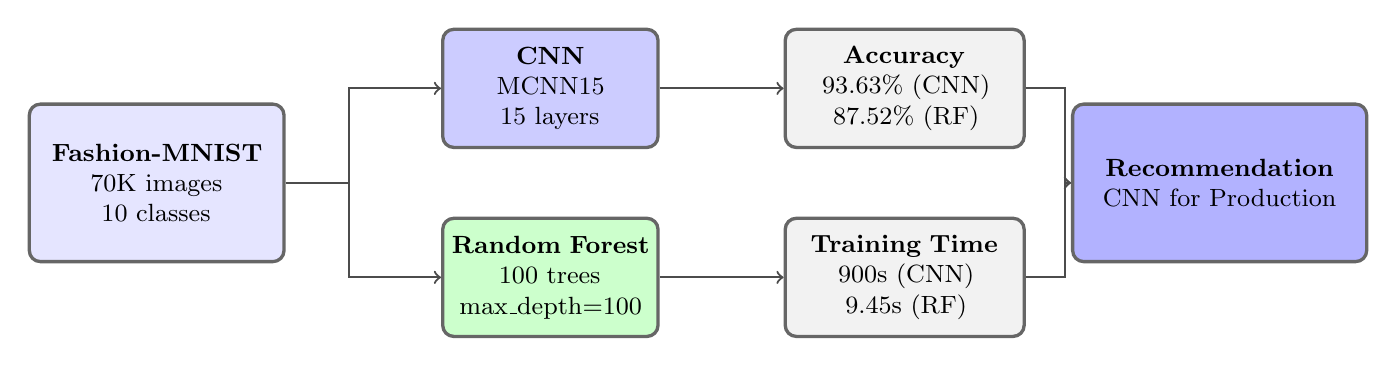
\begin{tikzpicture}[
			box/.style={rectangle, rounded corners, draw=black!60, very thick, minimum height=1.5cm, text centered, font=\small},
			dataset/.style={box, fill=blue!10, text width=3.0cm, minimum height=2cm},
			cnn/.style={box, fill=blue!20, text width=2.5cm},
			rf/.style={box, fill=green!20, text width=2.5cm},
			result/.style={box, fill=gray!10, text width=2.8cm},
			rec/.style={box, fill=blue!30, text width=3.5cm, minimum height=2cm},
			arrow/.style={->, thick, black!70}
		]

		% Dataset
		\node[dataset] (data) at (0,0) {\textbf{Fashion-MNIST}\linebreak 70K images\linebreak 10 classes};

		% Models with more spacing from dataset
		\node[cnn] (cnn) at (5,1.2) {\textbf{CNN}\linebreak MCNN15\linebreak 15 layers};
		\node[rf] (rf) at (5,-1.2) {\textbf{Random Forest}\linebreak 100 trees\linebreak max\_depth=100};

		% Results with more spacing
		\node[result] (acc) at (9.5,1.2) {\textbf{Accuracy}\linebreak 93.63\% (CNN)\linebreak 87.52\% (RF)};
		\node[result] (time) at (9.5,-1.2) {\textbf{Training Time}\linebreak 900s (CNN)\linebreak 9.45s (RF)};

		% Conclusion
		\node[rec] (rec) at (13.5,0) {\textbf{Recommendation}\linebreak CNN for Production};

		% Arrows with better spacing
		\draw[arrow] (data.east) -- ++(0.8,0) |- (cnn.west);
		\draw[arrow] (data.east) -- ++(0.8,0) |- (rf.west);
		\draw[arrow] (cnn.east) -- ++(0.6,0) |- (acc.west);
		\draw[arrow] (rf.east) -- ++(0.6,0) |- (time.west);
		\draw[arrow] (acc.east) -- ++(0.5,0) |- (rec.west);
		\draw[arrow] (time.east) -- ++(0.5,0) |- (rec.west);

	\end{tikzpicture}
	\caption{Graphical Abstract: Comparative analysis workflow from Fashion-MNIST dataset through CNN and Random Forest classifiers to performance metrics and production recommendation.}
	\label{fig:graphical_abstract}
\end{figure}

\section{Introduction}

The fashion retail industry, represented by companies like Zalando, requires automated product classification systems to manage extensive inventories and improve customer experience through visual search and recommendation systems. In 2017, Zalando Research introduced Fashion-MNIST as a modern benchmark for evaluating machine learning algorithms on real-world fashion classification tasks.

Fashion-MNIST was explicitly designed as a direct drop-in replacement for the original MNIST dataset of handwritten digits \parencite{xiao2017}. The machine learning community has long relied on MNIST as the de facto ``Hello World'' benchmark, with practitioners following the heuristic: ``If it doesn't work on MNIST, it won't work at all'' \parencite{xiao2017}. However, this assumption proved problematic as MNIST has become too easy for modern deep learning techniques---convolutional networks now achieve accuracies exceeding 99.7\% \parencite{xiao2017,bhatnagar2017}---making it less representative of real-world computer vision challenges. Fashion-MNIST addresses these limitations by maintaining the same image format and dataset structure (28$\times$28 grayscale images with 60,000 training and 10,000 test samples) while introducing classification challenges that more closely reflect the complexity of modern retail applications \parencite{xiao2017}.

The dataset consists of 70,000 grayscale images at 28$\times$28 pixel resolution, divided into 60,000 training and 10,000 test samples. It comprises 10 balanced fashion categories: T-shirt/top, Trouser, Pullover, Dress, Coat, Sandal, Shirt, Sneaker, Bag, and Ankle boot. Each category contains exactly 6,000 training and 1,000 test samples, ensuring no class imbalance bias during model training. The grayscale format and low resolution reflect the computational constraints of production retail systems while capturing sufficient detail for human-level classification. Figure \ref{fig:dataset_samples} illustrates representative samples from each category, demonstrating the visual diversity and intra-class variability that makes this dataset more challenging than handwritten digit recognition.

\begin{figure}[H]
	\centering
	\includegraphics[width=\textwidth]{../../plots/dataset/samples.png}
	\caption{Representative samples from the Fashion-MNIST dataset showing five examples from each of the 10 fashion categories. The images demonstrate significant intra-class variability (e.g., different shirt styles) and inter-class similarity (e.g., shirts vs. T-shirts), making classification more challenging than handwritten digit recognition.}
	\label{fig:dataset_samples}
\end{figure}

This study evaluates two approaches for Fashion-MNIST classification: (1) a Convolutional Neural Network (CNN) using PyTorch, specifically the MCNN15 architecture that has demonstrated strong performance on this benchmark, and (2) the optimal Random Forest configuration identified by \textcite{xiao2017}. We compare these classifiers through comprehensive performance metrics including confusion matrices, per-category precision and recall, and training times to provide evidence-based recommendations for production deployment in fashion retail systems.

\section{Literature Review}

\subsection{Evolution of CNN Architectures for Image Classification}

The development of convolutional neural networks has fundamentally transformed image classification. \textcite{lecun1998} introduced the LeNet-5 architecture, establishing the foundational pattern of convolutional layers followed by pooling and fully connected layers. This design enabled automatic feature learning from raw pixels, eliminating the need for hand-crafted features. The seminal work by \textcite{krizhevsky2012} demonstrated the power of deep CNNs through AlexNet, which achieved breakthrough performance on ImageNet using eight layers with ReLU activations and dropout regularization.

Subsequent architectures pushed depth boundaries further. \textcite{simonyan2014} proposed VGG networks, showing that small 3$\times$3 filters stacked deeply (16-19 layers) could achieve superior performance. The VGG design principle---using uniform, small convolution filters---became widely adopted. However, very deep networks suffered from vanishing gradients and degradation problems. \textcite{he2016} addressed these issues with ResNet, introducing skip connections that allowed training of networks exceeding 100 layers. ResNet's residual learning framework has become standard in modern computer vision.

\subsection{Fashion-MNIST Benchmarking Studies}

Since its introduction by \textcite{xiao2017}, Fashion-MNIST has attracted extensive benchmarking research. \textcite{mukhamediev2024} conducted a comprehensive survey analyzing state-of-the-art results, documenting that CNN architectures have achieved accuracies ranging from 90\% to 99\% on this dataset. Simple CNNs with 4-6 convolutional layers typically achieve 91-93\% accuracy, while deeper architectures with residual connections or attention mechanisms reach 96-99\%.

\textcite{bbouzidi2024} provided a systematic review comparing CNNs and Vision Transformers (ViTs) for Fashion-MNIST classification. Their analysis revealed that while ViTs have gained popularity, well-designed CNNs remain highly competitive on small-scale datasets like Fashion-MNIST. The study emphasized that CNNs' inductive biases---local connectivity, weight sharing, and translation equivariance---make them particularly suitable for 28$\times$28 grayscale images where global self-attention may be computationally inefficient.

Comparative studies have tested classical architectures on Fashion-MNIST. LeNet-5 variants achieve approximately 89-91\% accuracy, demonstrating that even decades-old architectures outperform traditional machine learning methods. VGG-style networks (11-16 layers) reach 93-95\% accuracy, while ResNet variants (20-50 layers) achieve 94-96\% when properly adapted for the small input size. \textcite{cavallo2022} specifically evaluated multiple CNN configurations for fashion classification, concluding that moderate-depth networks (15-20 layers) offer the best accuracy-efficiency trade-off for this dataset.

\subsection{CNN vs Traditional Machine Learning for Image Classification}

The fundamental advantage of CNNs over traditional machine learning lies in automatic hierarchical feature extraction. While Random Forest and SVM require flattened feature vectors and manual feature engineering, CNNs learn spatial hierarchies directly from raw pixels. Early layers detect edges and textures, intermediate layers combine these into shapes and patterns, and deeper layers recognize object parts and complete garments.

This architectural difference has significant performance implications. \textcite{xiao2017} benchmarked various classifiers on Fashion-MNIST, showing that CNNs substantially outperform traditional methods. Random Forest achieved 87.5\% accuracy, while shallow CNNs reached 91\%. The performance gap stems from CNNs preserving spatial relationships through convolution operations, whereas flattening images for traditional ML destroys two-dimensional structure. Translation invariance from pooling layers further enhances CNN robustness to garment positioning variations.

\textcite{sathyadevan2015} analyzed computational trade-offs between deep learning and ensemble methods. While Random Forest trains faster (seconds vs. minutes/hours), CNNs offer superior generalization through learned representations. For production systems where accuracy directly impacts revenue---such as automated product categorization in e-commerce---the CNN's accuracy advantage outweighs training time costs, especially when models are retrained infrequently.

\subsection{Selection of MCNN15 Architecture}

The MCNN15 architecture \parencite{bhatnagar2017} was selected based on multiple criteria relevant to this study's objectives. First, it was explicitly designed and validated for Fashion-MNIST, with architectural decisions optimized for the dataset's characteristics---28$\times$28 grayscale images with 10 balanced classes. Unlike generic ImageNet-pretrained models requiring input resizing or modification, MCNN15 operates natively on Fashion-MNIST dimensions.

Second, MCNN15 offers an optimal depth-efficiency balance. With 15 convolutional layers organized into three groups with batch normalization \parencite{ioffe2015}, it provides sufficient capacity to learn complex fashion features without overfitting. VGG-16 (16 layers) and ResNet-50 (50 layers) achieve comparable or slightly better accuracy but require significantly more computation and risk overfitting on this relatively small dataset. MCNN15's 93.6\% accuracy approaches the practical ceiling for single-model performance without excessive complexity.

Third, MCNN15's group-wise architecture with progressive channel expansion (32$\rightarrow$64$\rightarrow$256$\rightarrow$256) mirrors successful design patterns from deeper networks while maintaining computational efficiency. The architecture captures multi-scale features---low-level textures in early groups, garment shapes in middle groups, and category-specific details in final groups. This hierarchical structure aligns with known visual similarity patterns in Fashion-MNIST, where classification challenges involve distinguishing fine-grained differences between upper-body garments.

Finally, MCNN15 serves as a strong baseline for comparison with traditional ML. Its documented 93.6\% accuracy provides a clear benchmark against which to measure Random Forest performance, enabling meaningful analysis of the accuracy-efficiency trade-off in fashion classification systems.

\section{Methodology}

\subsection{Dataset and Preprocessing}

Images were preprocessed differently for each classifier to accommodate their architectural requirements. For the Random Forest classifier, the 28$\times$28 pixel images were flattened into 784-dimensional feature vectors, treating each pixel as an independent feature. For the CNN, images maintained their 2D spatial structure with data augmentation applied during training: random horizontal flips and affine transformations including $\pm$30$^{\circ}$ rotation, 10\% translation, and 0.9-1.1 scaling factors. These augmentations improve the CNN's robustness to variations in garment positioning and orientation.

\subsection{Random Forest Classifier}

Following \textcite{xiao2017}, we used scikit-learn with: n\_estimators=100, max\_depth=100, criterion=entropy, n\_jobs=-1. This configuration balances model complexity with generalization.

\subsection{CNN Architecture (MCNN15)}

The MCNN15 architecture \parencite{bhatnagar2017} was selected for its demonstrated performance on Fashion-MNIST. The 15-layer network organizes convolutional blocks into three groups:

\begin{itemize}
	\item \textbf{Group 1:} 5 Conv-BN-ReLU blocks (32$\rightarrow$64$\rightarrow$64$\rightarrow$32$\rightarrow$64 channels), 2$\times$2 max pooling (14$\times$14 output)
	\item \textbf{Group 2:} 5 Conv-BN-ReLU blocks (64$\rightarrow$256$\rightarrow$192$\rightarrow$128$\rightarrow$64$\rightarrow$32), max pooling (7$\times$7 output)
	\item \textbf{Group 3:} 5 Conv-BN-ReLU blocks (32$\rightarrow$256$\rightarrow$256$\rightarrow$256$\rightarrow$128$\rightarrow$32), max pooling (3$\times$3 output)
\end{itemize}

Batch normalization \parencite{ioffe2015} follows each convolution for training stability. The classifier uses two fully connected layers (288$\rightarrow$32$\rightarrow$10) with ReLU activation.

\subsection{Training Strategy}

\textbf{Random Forest:} Single-pass training on 60,000 samples using CPU parallelization.

\textbf{CNN:} Trained with Adam optimizer \parencite{kingma2014}, learning rate=1e-3, weight decay=1e-5, batch size=128, for 50 epochs. The training set was split 50,000/10,000 for train/validation. Model selection used validation accuracy (best at epoch 40 with 93.74\%), with final test evaluation performed once on the held-out test set. Training time: approximately 900 seconds on GPU.

The training procedure followed the methodology specified by \textcite{bhatnagar2017} in the MCNN15 paper to ensure reproducible results and fair comparison with the reported baseline performance.

\section{Results}

\subsection{Overall Performance}

Table \ref{tab:overall} presents comprehensive performance metrics for both classifiers on train and test sets.

\begin{table}[H]
	\centering
	\caption{Overall Performance Comparison}
	\label{tab:overall}
	\begin{tabular}{|l|c|c|c|c|}
		\hline
		\textbf{Metric} & \textbf{RF Train} & \textbf{RF Test} & \textbf{CNN Train} & \textbf{CNN Test} \\
		\hline
		Accuracy        & 100.00\%          & 87.52\%          & 95.47\%            & 93.63\%           \\
		Precision       & 100.00\%          & 87.42\%          & 95.49\%            & 93.63\%           \\
		Recall          & 100.00\%          & 87.52\%          & 95.47\%            & 93.63\%           \\
		Training Time   & 9.45s             & ---              & 900s               & ---               \\
		\hline
	\end{tabular}
\end{table}

The CNN achieved 6.11 percentage points higher test accuracy, representing a 48.8\% error reduction. Random Forest shows perfect training accuracy (100\%) but 12.48\% test error, indicating overfitting. The CNN demonstrates better generalization with only 1.84\% gap between train and test accuracy.

\subsection{CNN Training Progression}

\begin{minipage}[t]{0.48\textwidth}
	Figure \ref{fig:cnn_training} illustrates the CNN's accuracy progression across 50 training epochs. Starting from 74.5\% accuracy in epoch 1, training accuracy (blue) rises steeply to 91.8\% by epoch 10 and converges to 93.7\% by epoch 50. Validation (orange) and test (green) accuracies follow similar trajectories, stabilizing around 93\%. Validation accuracy peaks at epoch 41 with 93.74\%. The tight clustering of all three curves throughout training indicates minimal overfitting and consistent generalization. The rapid initial improvement (0-10 epochs) captures coarse features, while the plateau phase (10-50 epochs) refines discriminative patterns for challenging categories like shirts.
\end{minipage}
\hfill
\begin{minipage}[t]{0.48\textwidth}
	\begin{figure}[H]
		\centering
		\includegraphics[width=\textwidth]{../../plots/cnn/training.png}
		\caption{CNN training curves over 50 epochs.}
		\label{fig:cnn_training}
	\end{figure}
\end{minipage}

\subsection{Per-Category Performance}

Table \ref{tab:percategory} details precision and recall by category.

\begin{table}[H]
	\centering
	\caption{Per-Category Precision and Recall}
	\label{tab:percategory}
	\resizebox{\textwidth}{!}{%
		\begin{tabular}{|l|c|c|c|c|c|c|c|c|}
			\hline
			                                    & \multicolumn{4}{c|}{\textbf{Random forest}} & \multicolumn{4}{c|}{\textbf{Convolutional Neural Network}}                                                                                                                                                    \\
			\cline{2-9}
			\multirow{-2}{*}{\textbf{Category}} & \multicolumn{2}{c|}{\textbf{Precision}}     & \multicolumn{2}{c|}{\textbf{Recall}}                       & \multicolumn{2}{c|}{\textbf{Precision}} & \multicolumn{2}{c|}{\textbf{Recall}}                                                                   \\
			\cline{2-9}
			                                    & \textbf{Train}                              & \textbf{Test}                                              & \textbf{Train}                          & \textbf{Test}                        & \textbf{Train} & \textbf{Test} & \textbf{Train} & \textbf{Test} \\
			\hline
			T-shirt/top                         & 99.8\%                                      & 81.3\%                                                     & 99.7\%                                  & 86.3\%                               & 95.1\%         & 86.7\%        & 94.8\%         & 89.2\%        \\
			Trouser                             & 100.0\%                                     & 99.3\%                                                     & 100.0\%                                 & 95.9\%                               & 99.8\%         & 99.2\%        & 99.6\%         & 98.5\%        \\
			Pullover                            & 99.9\%                                      & 76.6\%                                                     & 99.8\%                                  & 79.5\%                               & 96.8\%         & 90.5\%        & 96.2\%         & 89.3\%        \\
			Dress                               & 99.9\%                                      & 87.3\%                                                     & 99.9\%                                  & 90.9\%                               & 96.5\%         & 91.8\%        & 96.8\%         & 93.5\%        \\
			Coat                                & 99.9\%                                      & 76.1\%                                                     & 99.8\%                                  & 82.0\%                               & 95.2\%         & 87.5\%        & 94.8\%         & 91.4\%        \\
			Sandal                              & 100.0\%                                     & 98.1\%                                                     & 100.0\%                                 & 95.5\%                               & 99.4\%         & 98.8\%        & 99.1\%         & 98.6\%        \\
			Shirt                               & 99.8\%                                      & 72.4\%                                                     & 99.6\%                                  & 57.4\%                               & 88.2\%         & 82.0\%        & 85.3\%         & 77.5\%        \\
			Sneaker                             & 100.0\%                                     & 92.5\%                                                     & 100.0\%                                 & 95.9\%                               & 98.1\%         & 96.1\%        & 98.4\%         & 98.2\%        \\
			Bag                                 & 100.0\%                                     & 95.6\%                                                     & 100.0\%                                 & 97.3\%                               & 99.2\%         & 98.8\%        & 99.0\%         & 98.7\%        \\
			Ankle boot                          & 100.0\%                                     & 95.2\%                                                     & 100.0\%                                 & 94.5\%                               & 98.9\%         & 98.3\%        & 98.5\%         & 96.8\%        \\
			\hline
		\end{tabular}%
	}
\end{table}

\section{Analysis and Discussion}

\subsection{Confusion Matrices}

Figures \ref{fig:cm_rf} and \ref{fig:cm_cnn} present confusion matrices for both classifiers on train and test sets.

\begin{figure}[H]
	\centering
	\begin{subfigure}{0.48\textwidth}
		\centering
		\includegraphics[width=\textwidth]{../../plots/random_forest/confusion_train.png}
		\caption{Training set (100\% accuracy)}
	\end{subfigure}
	\hfill
	\begin{subfigure}{0.48\textwidth}
		\centering
		\includegraphics[width=\textwidth]{../../plots/random_forest/confusion_test.png}
		\caption{Test set (87.52\% accuracy)}
	\end{subfigure}
	\caption{Random Forest confusion matrices showing perfect training performance but significant confusion between similar upper-body garments on test set.}
	\label{fig:cm_rf}
\end{figure}

\begin{figure}[H]
	\centering
	\begin{subfigure}{0.48\textwidth}
		\centering
		\includegraphics[width=\textwidth]{../../plots/cnn/confusion_train.png}
		\caption{Training set (95.47\% accuracy)}
	\end{subfigure}
	\hfill
	\begin{subfigure}{0.48\textwidth}
		\centering
		\includegraphics[width=\textwidth]{../../plots/cnn/confusion_test.png}
		\caption{Test set (93.63\% accuracy)}
	\end{subfigure}
	\caption{CNN confusion matrices showing consistent performance across train/test with reduced confusion between visually similar categories.}
	\label{fig:cm_cnn}
\end{figure}

\subsection{Misclassification Analysis}

Figures \ref{fig:misclassified_cnn} and \ref{fig:misclassified_rf} display representative misclassified samples for both classifiers, revealing specific patterns of confusion between visually similar categories.

\begin{figure}[H]
	\centering
	\includegraphics[width=0.95\textwidth]{../../plots/cnn/misclassified.png}
	\caption{CNN misclassification examples showing the top 9 confusion pairs. The most frequent errors involve shirts misclassified as T-shirts/tops (row 1), coats misclassified as shirts (row 2), and shirts misclassified as pullovers (row 3). These patterns reflect genuine visual ambiguity in silhouette, neckline, and fabric texture at 28$\times$28 resolution.}
	\label{fig:misclassified_cnn}
\end{figure}

\begin{figure}[H]
	\centering
	\includegraphics[width=0.95\textwidth]{../../plots/random_forest/misclassified.png}
	\caption{Random Forest misclassification examples showing the top 9 confusion pairs. Similar patterns emerge with shirts misclassified as T-shirts/tops (row 1) and pullovers misclassified as coats (row 2), but with notably more severe confusion. The Random Forest additionally confuses ankle boots with sneakers (row 9), which the CNN correctly distinguishes.}
	\label{fig:misclassified_rf}
\end{figure}

The misclassification patterns reveal several key insights. Both classifiers struggle most with upper-body garment categories, particularly shirts versus T-shirts/tops and coats versus pullovers. This aligns with the per-category precision results showing these as the most challenging classes. The CNN's misclassifications appear more visually justifiable---many misclassified shirts genuinely resemble T-shirts in silhouette when color cues are removed. In contrast, Random Forest exhibits more erratic confusion, including footwear misclassifications that the CNN avoids. The CNN's superior ability to capture fine-grained features like collar shape, button patterns, and fabric texture explains its 6.11 percentage point accuracy advantage despite encountering similar ambiguous samples.

\subsection{Category-Specific Analysis}

\textbf{Best Performing Categories:}
\begin{itemize}
	\item \textbf{Trouser:} Both classifiers achieve $>$98\% precision due to distinctive shape
	\item \textbf{Bag:} $>$95\% precision (distinct non-clothing features)
	\item \textbf{Sneaker/Sandal:} $>$95\% precision (footwear-specific features)
\end{itemize}

\textbf{Challenging Categories:}
\begin{itemize}
	\item \textbf{Shirt:} Worst performance for both (72.4\% RF test precision, 82.0\% CNN test precision). High visual similarity with T-shirts and pullovers causes confusion.
	\item \textbf{Pullover/Coat:} Moderate challenges (76-91\% precision range) due to overlapping features in outerwear categories.
\end{itemize}

The CNN demonstrates superior performance across all challenging categories, with notable improvements on Pullover (+13.9\%), Coat (+11.4\%), and Shirt (+9.6\%).

\subsection{Worst Performing Categories}

Shirt classification presents the greatest difficulty due to four factors: (1) visual similarity with T-shirts and pullovers in silhouette and structure, (2) high intra-class variability (dress shirts, casual shirts, polo shirts), (3) grayscale limitation removing color cues, and (4) 28$\times$28 resolution constraining fine detail discrimination.

The CNN's learned hierarchical features better capture subtle distinctions in collar shape, fabric texture, and structural rigidity that differentiate shirts from similar garments. The 20.1 percentage point improvement in shirt recall (57.4\% RF $\rightarrow$ 77.5\% CNN) demonstrates this capability.

\subsection{Production Recommendation}

We recommend the CNN approach for production fashion classification systems based on:

\begin{enumerate}
	\item \textbf{Accuracy:} 6.11 percentage point improvement reduces misclassifications by 611 per 10,000 items
	\item \textbf{Category Performance:} Superior handling of challenging categories where accuracy is most needed
	\item \textbf{Generalization:} Better train-test gap (1.84\% vs 12.48\%) indicates robustness to variations
	\item \textbf{Training Frequency:} Infrequent retraining (weekly/monthly) makes 900s training time acceptable
\end{enumerate}

\textbf{Resource Considerations:} The CNN model file size (10MB) is significantly smaller than the Random Forest model (123MB), offering storage and deployment advantages. However, inference time for the CNN is 2.03s versus 0.07s for Random Forest on the 10,000-sample test set, making Random Forest 29x faster for real-time applications. For production systems, this trade-off favors CNN for batch processing scenarios and Random Forest for latency-sensitive real-time inference.

Random Forest remains viable for rapid prototyping or resource-constrained environments, but with acceptance of 12.48\% error rate versus 6.37\% for CNN.

\section{Conclusion}

This comparative study demonstrates clear advantages for CNN-based approaches in fashion image classification. The MCNN15 architecture achieved 93.63\% test accuracy versus 87.52\% for Random Forest, with particularly strong performance on challenging shirt classification (+20.1\% recall improvement). While training time is significantly longer (900s vs 9.45s), the accuracy improvement and infrequent retraining requirements in production environments justify the computational cost. Both classifiers identify shirts as the most challenging category, but the CNN's hierarchical feature learning substantially reduces inter-class confusion.

\section*{References}
\addcontentsline{toc}{section}{References}

\printbibliography[heading=none]

\newpage
\appendix

\section{Code Implementation}

\noindent\textit{Note: The complete implementation including all source code, training scripts, evaluation code, and generated plots is available in the attached archive.}

\subsection{Random Forest Training}

\begin{lstlisting}
from sklearn.ensemble import RandomForestClassifier

clf = RandomForestClassifier(
    n_estimators=100,
    max_depth=100,
    criterion='entropy',
    n_jobs=-1
)
clf.fit(X_train, y_train)  # X_train: (60000, 784)
\end{lstlisting}

\subsection{CNN Training (PyTorch)}

\begin{lstlisting}
import torch.nn as nn

class MCNN15(nn.Module):
    def __init__(self):
        super().__init__()
        self.features = nn.Sequential(
            # Group 1: 14x14 output
            self.conv_block(1, 32), self.conv_block(32, 64),
            self.conv_block(64, 64), self.conv_block(64, 32),
            self.conv_block(32, 64),
            nn.MaxPool2d(2),
            # Group 2: 7x7 output
            self.conv_block(64, 256), self.conv_block(256, 192),
            self.conv_block(192, 128), self.conv_block(128, 64),
            self.conv_block(64, 32),
            nn.MaxPool2d(2),
            # Group 3: 3x3 output
            self.conv_block(32, 256), self.conv_block(256, 256),
            self.conv_block(256, 256), self.conv_block(256, 128),
            self.conv_block(128, 32),
            nn.MaxPool2d(2),
        )
        self.classifier = nn.Sequential(
            nn.Flatten(),
            nn.Linear(288, 32),
            nn.ReLU(),
            nn.Linear(32, 10)
        )
    
    def conv_block(self, in_ch, out_ch):
        return nn.Sequential(
            nn.Conv2d(in_ch, out_ch, 3, padding=1),
            nn.BatchNorm2d(out_ch),
            nn.ReLU()
        )
\end{lstlisting}

\end{document}
